\chapter{Modular Run-Time}

\section{Objectives}

When thinking about creating a run-time from the scratch, one has to think mainly about two things:

\begin{itemize}
  \item{\bf{Speed}} The run-time is the core of every app that uses it. The speed of the apps using the run-time is greatly dependent on the speed of the run-time, the method dispatch in particular.
  \item{\bf{Flexibility}} The run-time should be as flexible as possible. It should be easy to port the framework to other platforms, and even to kernel space. You should be able to add custom features to the run-time without modifying the run-time's source code - just adding another source code file and possibly registering it on the fly without the need to even recompile the run-time.
\end{itemize}

The main objective of this work is to create a prototype of a completely new run-time that will have no dependencies on any external libraries, not even the POSIX layer, thus allowing the developer to easily set up his own run-time from different modules.

Also, no constructs that require any OS support (dynamic loader, standard OS libraries, etc.) will be used. This means, that constructs such as \verb=static __thread= (which creates a new copy of the variable declared for each thread created) or \newline{} \verb=__attribute__((constructor))= (which marks the function to be called by the dynamic loader right after the binary has been loaded) can be used either.

In its way, the run-time will be a bare skeleton, which will be ready to be extended for a particular system. As I have decided not to use any compiler-specific extensions, the \verb=constructor= attribute in particular, a question arises, who or what will initialize the run-time.

On systems that do support the constructor functions, this can be easily solved by compiling the run-time with an additional file which will declare and implement a constructor, as can be seen in the \verb=posix.c= file, which is included with the run-time as an extra, which demonstrates how to add support for your operating system.

In a real-world scenario, of course, it cannot be assumed that every program's \verb=main= function will start by feeding the run-time with necessary function pointers and calling the run-time initializer. For example, on \verb=*nix=\footnote{Most Unix-based systems, cannot be guaranteed that this will work on all of the systems.} systems, this can be easily solved by compiling the library with a single \verb=.c= file which has a function populating the setup structure with system-specific functions. As can be seen in the aforementioned \verb=posix.c= file.

This only solves a half of the problem. Who is responsible for calling the \verb=_objc_posix_init= function if your system doesn't support constructor functions? If it is possible to tie the run-time with the OS more tightly, the answer is the dynamic loader. If this isn't the case, then a few options emerge:

\begin{itemize}
  \item{\bf{Use a special \verb=main= function}} Instead of implementing the main function in the program itself, implement it inside the run-time and make it call an external \verb=objc_main= function, which would get to be implemented in the program. It is similar to start of a C program, where the \verb=start= function is called, which initializes some C global variables and then calls the \verb=main= function.
  \item{\bf{Add hooks to class registration}} Second option is to add a check into the class creating/registering functions if the run-time has already been initialized (a global variable may be used for this) and if not, call the initializing function and continue. Class registration function seems like a good place to add such a hook as it doesn't make sense to call any other functions if no classes have been registered with the run-time. Also, such a check does cost something (an \verb=if= statement), so it is not suitable for any function that gets called more often.
\end{itemize}

Now that the initialization has been figured out, even on systems that do not support constructors, another question comes up - what about the on-the-fly customization? What if I want to customize the run-time at the beginning of my program? Here's a few examples a person might want to change:

\begin{itemize}
\item{\bf{Example 1: Lock-less run-time}}
In a single-threaded application (or applications, where you know that Objective-C code will be used only in one thread), there is no need for any locking whatsoever. All of the existing implementations require some locking, even though they are using read-lock-free structures, such as sparse arrays that do not support deleting.

But even so, any \verb=@synchronized(obj)= code is translated to actually lock a mutex associated with \verb=obj=, be it either a mutex from a lock pool in the traditional run-times, or a mutex that is associated just with \verb=obj= in the \'Etoil\'e run-time. This can speed up both loading of the application and code execution.

\item{\bf{Example 2: Kernel usage}}

To get the existing run-times working in a kernel of an operating system might be tricky, depending on how much the kernel is POSIX-compatible. But even so, the \verb=malloc= functions and others usually are just wrappers around kernel allocators, which slows down allocation of all structures within the run-time.

Using the modular run-time, it is be possible to change the allocator with a simple function-pointer assignment.

\item{\bf{Example 3: Benchmarking}}

The modularity that will be introduced by this work will allow anyone to explore changes in the speed of the run-time simply by changing internal data structures used to hold the class list, selector list and caching. This may help the future development of the run-time.

\end{itemize}

Logically, there needs to be some sort of a line after which the run-time cannot be modified as it would lead to inconsistency - for example changing the deallocator after some objects have been already allocated may lead to memory leaks or crashes as the new deallocator will not recognize that particular memory. The following section describes how to set up the run-time.

\section{Run-time Setup}

As has been mentioned before, the run-time has been designed to be as flexible as possible. This means that all possible dependencies had to be removed, as well as all assumptions about the underlying OS, or whether the run-time is running in user space, or kernel space.

The run-time, however, needs a way to allocate memory, locks, and so on, which are system-specific tasks. The intention behind this run-time is to completely separate these dependencies, so that porting the run-time to another platform is as easy as providing a single file containing all the necessary resources.

There are basically two ways of doing so:

\begin{itemize}
\item{\bf{Inline Functions}}
The first one is very similar to what the other run-time implementations have done - create a header file that contains multiple static inline functions that implement all the OS-specific calls required by the run-time.

This approach to the platform-independence problem has one advantage and one disadvantage. The obvious disadvantage is that you can perform compile-time changes only. Once the run-time has been compiled, there is no way to change, for example, the allocator without performing some wild hackery exchanging the \verb=malloc= function pointer using the dynamic loader API.

The advantage, on the other hand, is definitely speed. There is no extra cost associated with calling these system APIs as the functions get inlined.

\item{\bf{Function Pointers}}
Another approach is to create a setup structure that consists of function pointers, which are then called by the run-time. This has the opposite advantages and disadvantages as inlining functions.

The advantage is that the run-time can be compiled without knowing the functions at all and then every program can decide which allocators to use, etc. Or if there is enough support from the dynamic loader, the dynamic loader can decide which functions to use to populate the run-time setup based on some binary flags.

The disadvantage here, on the other hand, is speed. While the function itself has to be called anyway, it is possible that the function types used in the run-time do not match function types in your system. You then need to create a proxy function that converts the parameters.

For example, the read/write lock functions are made to be compatible with the POSIX \verb=pthread_rwlock_*= functions (as can be seen in \verb=extras/posix.c=), which return an \verb=int= containing a possible error value, or zero if the call was successful. In the same manner, the run-time may assume that if the function pointer returns zero, the call was successful. If the OS you are porting the run-time to doesn't return anything, or returns a different value than zero for success, you need to create a proxy function that calls the system function and then returns some value accordingly. This, however, costs an extra function call.

\end{itemize}

Assuming that function pointers are used, you might want to disable all locks in your program as has been described in \textbf{Example 1} above. Even though most operating systems no-op all mutex-related function unless the program is running as multi-threaded. You may, however, be running a multi-threaded application with Objective-C code running in just one thread. Then it may be useful to no-op all the locking functions manually.

If there already is a function that fills all the function pointers, like the one in the \verb=posix.c= example, you need to modify the mutex pointers after the \verb=_objc_posix_init()= is called, as otherwise your change to the function pointers would get overwritten, yet before \verb=objc_runtime_init()= is called, as afterwards, any attempt to modify the run-time setup will result in abort.

Again, several options emerge:

\begin{itemize}
  \item{\bf{With compiler and dynamic loader support}} If enough support is possible from both, just like the \verb=constructor= attribute, other attributes, such as \verb=objc_constructor= and \verb=objc_modifier= could be used, where the constructor would get called first, in our example the \verb=_objc_posix_init= and the modifiers would follow.
  \item{\bf{Without compiler and dynamic loader support}} As the previous option requires a lot of support from both the compiler and dynamic loader, it is unlikely to be used in less common operating systems, which this work is trying to target. For this reason, the run-time supports registering initializer functions that get called within \verb=objc_runtime_init=. Because the run-time has no way to allocate new memory, the number of such initializer functions needs to be limited to 32.
  
  This, again, poses a question when to call \verb=objc_runtime_init=. And the answer is simple. The run-time places a check in the \verb=objc_class_create= function and if the run-time hasn't been initialized, it gets initialized. So what if you call another function before the initialization? The program is likely to crash since it doesn't make much sense to call any other function without having registered at least one class.
  
  Note though that this is only to support systems with absolutely no support of anything described above, where the user himself would otherwise need to call the \verb=objc_runtime_init= function at the beginning of \verb=main= - which he still can, but it is redundant. If, however, for whatever reason, it is required to init the run-time at another time, it is possible to just call the \verb=objc_runtime_init= function manually. It can be called multiple times, however, only calling it the first time does anything. Note that registering an initializer after the runtime has been initialized aborts the program, though.
\end{itemize}

\subsection{Implementation}

The run-time prototype that is part of this work is designed to support both solutions - function pointers and static inline functions. Hence if you decide that you want to choose speed over flexibility and dynamic nature of the run-time, you can do so.

The key to this is the \verb=os.h= header file. An \verb#if-#else= divides the file into two parts, one for the inlining support, second one for the function pointers support.

When compiling the run-time, you can switch between these two simply by redefining the \verb=OBJC_USES_INLINE_FUNCTIONS= value - \verb=0= for function pointers, \verb=1= for inline functions. This can be done in the \verb=Makefile= as can be seen in the sample \verb=Makefile= supplied.

\paragraph{Inlining}

The first part of the \verb=os.h= header file is the part that should be used for static inline functions. A rough sketch of how this should be used has been included:

\begin{verbatim}
#if TARGET_MY_OS
  #include "os-my-os.h"
#else
  #error "This OS isn't supported at the moment."
#endif
\end{verbatim}

You should hence create your own header file for that particular OS and include it in the run-time source files. The obvious disadvantage here is that you need to supply all necessary functions at the compile time.

The following list of functions needs to be defined:

\begin{itemize}
  \item{\bf{objc\_alloc}} Memory allocator.
  \item{\bf{objc\_zero\_alloc}} Memory allocator that fills the allocated memory with zeroes.
  \item{\bf{objc\_dealloc}} Memory deallocator.
  \item{\bf{objc\_abort}} Aborts the executions of the program.
  \item{\bf{\emph{objc\_log}}} Logs supplied format string.
  \item{\bf{objc\_rw\_lock\_create}} Creates a read-write lock.
  \item{\bf{objc\_rw\_lock\_rlock}} Locks the lock as read-only.
  \item{\bf{objc\_rw\_lock\_wlock}} Locks the lock as read/write.
  \item{\bf{objc\_rw\_lock\_unlock}} Unlocks the lock.
  \item{\bf{objc\_rw\_lock\_destroy}} Deallocates the lock.
  \item{\bf{\emph{objc\_class\_holder\_create}}} Creates a structure that registers classes.
  \item{\bf{\emph{objc\_class\_holder\_insert}}} Adds a class pointer to the structure.
  \item{\bf{\emph{objc\_class\_holder\_lookup}}} Looks up a class pointer for name.
  \item{\bf{\emph{objc\_selector\_holder\_create}}} Creates a structure that registers selectors.
  \item{\bf{\emph{objc\_selector\_holder\_insert}}} Inserts a selector.
  \item{\bf{\emph{objc\_selector\_holder\_lookup}}} Looks up a selector.
  \item{\bf{\emph{objc\_array\_create}}} Creates an array.
  \item{\bf{\emph{objc\_array\_append}}} Appends an item to an array.
  \item{\bf{\emph{objc\_array\_get\_enumerator}}} Returns an array enumerator.
  \item{\bf{\emph{objc\_cache\_create}}} Creates a cache for dynamic dispatch.
  \item{\bf{\emph{objc\_cache\_destroy}}} Destroys the cache structure.
  \item{\bf{\emph{objc\_cache\_fetch}}} Fetches a method for selector.
  \item{\bf{\emph{objc\_cache\_insert}}} Inserts a method into the cache.
\end{itemize}

When using static inline functions, all of these need to be implemented. To use the default implementation of functions that are marked italic in the list above, you may use the \verb=array-inline.h= and \verb=holder-inline.h= header files that are included in the \verb=extras= directory.

For a detailed description of each function, see the section about function pointers.

\paragraph{Function Pointers}

If you decide to use function pointers, you don't need to modify the run-time source code at all. The second part of the \verb=os.h= header file is filled with \verb=#define=s that fetch the corresponding function pointer. For example:

\begin{verbatim}
#if OBJC_USES_INLINE_FUNCTIONS

  /* ... */

#else

  #include "private.h"

  #define objc_alloc objc_setup.memory.allocator

  /* ... */

#endif

\end{verbatim}

The run-time defines a private \verb=objc_setup= global variable in \verb=runtime.c= and exports it in \verb=private.h=:
 
\begin{verbatim}
objc_runtime_setup_struct objc_setup;
\end{verbatim}

While the user has no direct access to this structure as it is exported in a private header (and the \verb=os.h= header doesn't get exported as well), the run-time itself can access it directly for the sake of speed to eliminate unnecessary function calls that would serve just as proxy calls. The user doesn't have a direct access to the structure only as a security precaution, so that the structure cannot be modified from the outside during the program execution, but the user is free to get the setup structure using the \verb=objc_runtime_get_setup= function, which copies over the whole setup structure. The user can then cache this structure for performance, so that he doesn't have to fetch it each time he wants to access a run-time function.

You can view the structure below:

\begin{verbatim}
typedef struct {
  objc_setup_memory_t memory;
  objc_setup_execution_t execution;
  objc_setup_sync_t sync;
  
  objc_setup_logging_t logging;
  
  objc_setup_class_holder_t class_holder;
  objc_setup_selector_holder_t selector_holder;
  objc_setup_array_t array;
  objc_setup_cache_t cache;
} objc_runtime_setup_t;
\end{verbatim}

The structure contains a set of structures, each containing a set of related functions. For example, the \verb=objc_setup_memory_t= structure:

\begin{verbatim}
typedef struct {
  objc_allocator_f allocator;
  objc_deallocator_f deallocator;
  objc_zero_allocator_f zero_allocator;
} objc_setup_memory_t;
\end{verbatim}

This allows the modularity of the run-time. One can, at the beginning of his program (as has been described above), modify all of those pointers using setter functions declared in \verb=ftypes.h=. After the runtime has been initialized, however, the whole structure is sealed off changes using those setter functions to prevent any data corruption (as some data structures may be already initialized, changing these functions would most likely lead to bad memory access crashing the program). Using any of the setter functions after the run-time has been initialized will cause the program to be aborted.

A description of each section of the setup structure can be found below:

\paragraph{Memory}

As the run-time needs new memory for dynamic object creation, an allocator is needed. All existing run-times use \verb=malloc=, which, however, ties them to systems that use malloc.

The Modular Run-Time lets you specify your own allocator, which can, for example, be just a wrapper around \verb=malloc= adding some debug logging, or a completely different allocator, e.g.\ a kernel allocator as has been mentioned before. It can also be just the \verb=malloc= function itself, as the function type takes just one argument - the size of the memory required and returns a \verb=void*= pointer.

Sometimes, the memory acquired should be filled with zeros - just as the \verb=calloc= function would do, however, it is called \verb=zero_allocator= in this run-time. Also, unlike the \verb=calloc= function, the \verb=zero_allocator= takes only one argument - the size of memory. It can be easily declared as \verb=calloc(1, size)=.

When the run-time is done with memory it has allocated, it will deallocate it using the deallocate function, which has the same signature as the POSIX \verb=free= function.

\paragraph{Execution}

This part of the structure contains function pointers (in current version of the run-time only one) to functions dealing with the execution of the program itself - it is commonly said that there is no software without bugs - hence it is sometimes necessary to abort the program execution if the program gets into an inconsistent point, or a point where illegal arguments are passed to the environment (for example, setting the run-time setup structure to NULL), hence it contains an \verb=objc_abort= function, which aborts the run of the program. Unlike the regular \verb=abort= function, this one takes an additional argument - the reason why it is being aborted.

\paragraph{Synchronization}

The synchronization structure consists of substructures, or in current state a single one - declaring functions related to read-write locks - it is possible in the future additional synchronization-related functions, such as mutex, condition variables, etc.

\subparagraph{Read-Write Locks} The run-time currently uses only read-write locks to prevent concurrent writes to structures, which are mostly read-lock-free. The structure contains functions that create locks, dealloc them, r/w lock them or unlock them. The locking and unlocking functions are compatible with \newline{}\verb=pthread_rwlock_*= functions.

\paragraph{Logging}

In a very few cases, the run-time logs some information, that is mostly useful to an Objective-C developer, to see what went wrong. For example, when creating a class with the same name as an existing class, a message is logged that the class with this name already exists. The logging function is compatible with \verb=printf= and by default is filled with a no-op function, so you don't necessarily need to include a logging function in your run-time setup, if you don't want to see any log messages from the run-time.

\paragraph{Class Holder}

The run-time needs to keep track of all classes that are registered with it. To do so, it needs to keep a list in some data structure. As the run-time is designed to be flexible, it doesn't matter what data structure at all.

There is a defined data type \verb=objc_class_holder= which, however, is only a retyped \verb=void *=. The functions included in this structure need to be able to create such a structure, store a class pointer in it and look up a class pointer for a name, where, of course, speed matters as this class lookup function is used whenever a class method is called.

The run-time provides a default implementation of this structure, a very simple hash table with a constant number of fields for the simplicity. It should be most likely replaced by some more sophisticated structure if the run-time were to be used in an environment with hundreds of classes.

\paragraph{Selector Holder}

Just like with classes, the run-time needs to keep track of selectors, for a simple reason - if there is only one selector of the same name within the run-time, you can hash the pointer (when looking up method implementations later on in a cache), instead of reading the selector's name over and over again.

\paragraph{Arrays}

A lot of the code of the traditional run-times is riddled with code that takes care of consistency of dynamically growing arrays (or rather arrays of arrays) - there's a lot of duplicate code for functions related to lists of methods, protocols, etc.\ on each class.

This run-time declares a \verb=objc_array= type, which is again just a retyped \verb=void *=, but can be implemented in any possible way. The run-time includes a working implementation of such an array and installs these function pointers at initialization, unless other pointers are provided.

The default implementation is a linked list, which keeps track of its first and last object. It also includes a lock for insertion, however, as no delete operation is allowed, the lock doesn't need to be locked for reading.

To enable fast iteration over the array, an enumerator is returned, which contains a \verb=next= field, pointing to the next node. If your implementation does not use a linked list, it is a good idea to store the items in such a wrapper anyway and link them together, so that the run-time can iterate over your structure in a fast manner without knowing any details about its internal structure and implementation.

\paragraph{Cache}

As has been noted several times before, almost any language with dynamic dispatch uses some sort of a cache so that it doesn't have to climb the whole class hierarchy to find a method implementation of a method that is only implemented on the root class.

The caching mechanism is described in a greater detail in the Caching section below. 

If you want to disable the caching mechanism altogether, just replace the cache creator and fetch functions with functions that return \verb=NULL=, and the insert and destroy functions with a no-op function.

\section{Class}

At the core of the run-time lies a structure representing a class. Like the \'Etoil\'e run-time, this run-time doesn't provide a class pair - a class and its meta-class, but only a single class object that contains class methods as well. While it abandons the Smalltalk similarities, it provides greater flexibility, allowing the Objective-C class structure to be used for other languages as well.

\subsection{Structure of a Class}

The class structure begins with an \verb=isa= pointer, which points to itself - a class is hence its own instance. This allows a quick detection of a class in the method dispatch - \verb+obj->isa == obj+ - macros \verb=OBJC_OBJ_IS_CLASS= and \newline{}\verb=OBJC_OBJ_IS_INSTANCE= are included.

\begin{figure}[htbp] 
  
    \begin{verbatim}
      struct objc_class {
        Class isa;
        Class super_class;
        char *name;
        
        objc_array class_methods;
        objc_array instance_methods;
        
        objc_array ivars;
        
        objc_cache class_cache;
        objc_cache instance_cache;
        
        unsigned int instance_size;
        struct {
          BOOL in_construction : 1;
        } flags;
      };
    \end{verbatim}

  \centering{}
  \caption{Class structure.}
  \label{fig:class_struct}
\end{figure}

The \verb=isa= pointer is followed by a pointer to the super class, or \verb=Nil= in case the class is a root class. Name of the class is followed.

Next, class and instance methods are listed. Each of the \verb=objc_array= structures contains a C-style list of \verb=Method= pointers. In other words, each item of the array is actually a \verb=Method *= array. Thanks to this, it is easy to add new methods in bulk - simply append the \verb=Method *= array to the \verb=objc_array=. This is generally how other run-times handle the method lists.

The ivars are directly listed in the \verb=objc_array= as ivar lists, unlike the method lists, are sealed after the class has been emph\{finished} (a step, where the run-time is informed that you do not intend to modify the class anymore and that it should be marked as ready for use - Apple calls this \emph{registering\ a\ class\ pair}), because adding an ivar is likely to change the size of the instances and most importantly of the class' subclasses. Adding methods on the fly, on the other hand, is a valid and used practice.

The class and instance caches will be explained in length in the Caching section that follows this section.

Instance size marks the size of the class' instances, yet doesn't include the space required by class extensions, which are described later, since the class structure may be loaded from a module, which doesn't know about installed class extensions.

A bitfield \verb=flags= follows, which includes a number of flags about the class. In particular, if it is still in construction - i.e.\ hasn't been \emph{finished} yet. Another flags might be included, such as if the class itself implements a \verb=+initialize= method, if such a method has been called, etc.

\section{Dynamic Dispatch and Caching}

The speed of the run-time really depends not that much on the speed of the lookup function itself (the function that climbs the class hierarchy looking for the method implementation in the method lists), which gets called only the first time a method with that particular selector, but depends mostly on the speed of the caching mechanism of the run-time.

Unlike Apple's implementation, the run-time doesn't handle the calling of the method implementation function itself, but just like the GCC run-time, or the \'Etoil\'e run-time, it looks up a \verb=Method= pointer, or an \verb=IMP= depending on your needs.

If you can assure inline caching, just like in the \'Etoil\'e run-time's proposal, then you should fetch the \verb=Method= pointer, which includes a \verb=version= field, which, just like in the \'Etoil\'e run-time gets incremented each time the \verb=Method= structure gets modified.

Using the inline caching, you can easily achieve near C-function-call speeds, as if the inline cache is indeed filled with a valid version of the \verb=Method=, the cost of the call over the direct C function call is one comparison for the selector and three comparisons of the cache properties - whether the \verb=Method= is not \verb=NULL= (note that in the \'Etoil\'e run-time, the structure isn't a method structure, but a \emph{slot}) - altogether, it is four pointer-equality comparisons and two \verb=if= statements. And that's it.

If the inline caching cannot be achieved, however, for example because the \verb=__thread= variables are unavailable on your system; or if the inline cache doesn't contain the correct version of the \verb=Method=, the mechanism needs to fallback to the traditional cache - a regular per-class cache - the class structure fields \verb=class_cache= and \verb=instance_cache=. Note that a class may implement a class and an instance method of the same name - the selector pointer is the same, but implementations differ (most likely). Hence the necessity of two caches per class (Apple and GCC run-times actually include two caches per class as well, though the fact is slightly hidden by the fact that each class is actually a class pair consisting of the class and meta-class objects).

When the inline cache is unavailable, or it misses, one of the following two methods should get called (a \verb=_super= alternative exists for \verb=super= calls):

\begin{verbatim}
extern Method objc_object_lookup_method(id obj, SEL selector);
extern IMP objc_object_lookup_impl(id obj, SEL selector);
\end{verbatim}

The first function returns the \verb=Method= pointer, so it should be used in case the compiler can generate inline caches. If it cannot, it is unnecessary to retrieve the \verb=Method= pointer, use the function fetching directly the method implementation, instead.

In either case, the look up function works like this:

\begin{enumerate}
  \item{\bf{Look inside the cache}} The function detects whether \verb=obj= is an instance of a class, or the class itself. Depending on that it looks inside the correct cache and if it results in a cache hit, the \verb=Method= is immediately returned. The cost of such call is \emph{dependent on the cache speed}.
  \item{\bf{Ask extensions}} As will be described later on, each class extension may supply its own lookup function, in case the extension can, for example, generate methods, or adds them via categories. If any extension finds a method implementation, it is then returned. Were there two such extensions that would implement this method, the extension that gets registered first is used (the extension list is iterated until an extension returns something other than \verb=NULL=). If any extension implements this method, it gets cached, so that the next time this method gets called on this class, the lookup will stop at the cache lookup.
  \item{\bf{Method lookup}} If the method implementation for this selector hasn't been cached yet, it is necessary to climb the class tree, looking into each class' method lists. If an implementation is found, it gets cached.
  \item{\bf{Forwarding}} Now, we are at a point where the method isn't cached, isn't implemented by any class extension, not the class itself or one of its superclasses. The modular run-time introduces a simplified forwarding mechanism, which gives the object a chance to handle the unrecognized selector. This forwarding mechanism is described in the next section.
  \item{\bf{Abort}} If the method hasn't been found and the class doesn't implement the forwarding mechanism, or the forwarding mechanism rejects this selector, the program is aborted.
\end{enumerate}

In its sense, the idea behind the caching is very simple and would be indeed very simple, if we wouldn't have to think about the following scenario, where \verb=Class3= is subclass of subclass of \verb=Class2=, which is subclass of \verb=Class1= and \verb=-doSomething= is a method implemented \emph{only} on \verb=Class1=:

\begin{enumerate}
  \item{\bf{\verb=Class2= and \verb=Class3= get instantiated}} An instance of both \verb=Class2= and \verb=Class3= gets created. Let's call those \verb=instance2= and \verb=instance3=.
  \item{\bf{Method \verb=doSomething= gets called on both \verb=instance2= and \verb=instance3=}} This results in caching the method implementation on both \verb=Class2= and \verb=Class3=, while the method itself is only implemented on their superclass \verb=Class1=.
  \item{\bf{Method \verb=doSomething= gets added to \verb=Class2=}} Either using \newline{}\verb=objc_class_add_instance_method=, or by adding a class category, the \verb=doSomething= method gets added to \verb=Class2=. Now, however, if \verb=instance2= or \verb=instance3= were to be called the \verb=doSomething= method, the cache would still point to the method implementation of \verb=Class1=.
\end{enumerate}

This presents a small hiccup on the easiness of the cache implementation as this scenario requires caches of \verb=Class2= and \verb=Class3= to be flushed. Note, though, that as the cache caches the whole \verb=Method= pointer, hence simply changing the method implementation pointer (the \verb=IMP=) doesn't require any cache flushing.

The question remains: how to flush the class cache. One might say that simply removing all cache entries is sufficient - in a single-threaded environment, this is indeed true. In a multi-threaded environment, this isn't the case as the cache may be read at the same time as it is being cleared.

While this could be overcome by locking the structure, it would require all readers to lock the read lock as well, which is, unfortunately, an unbearable cost as it would slow down the dynamic dispatch multiple times.

The solution to create a new cache structure, replace it in the \verb=Class= structure and keep the old cache structure alive as there still may be readers somewhere in the structure.

The question is, how long should the old structure be kept alive? This is up to the cache structure implementation. The modular run-time requires a function of type \verb=objc_cache_mark_to_dealloc_f= which should mark the cache structure as 'unnecessary' and that it should be deallocated at the first safe opportunity.

Apple's implementation solves this by looking at each thread's \verb=PC=/\verb=IP=/\verb=RIP= register and comparing it with the ranges of address of all functions that may be reading from the cache. In particular, those methods are listed in a global variable called \verb=objc_entryPoints= declared in the same assembly source file as the \verb=objc_msgSend= functions. The default implementation supplied with the modular run-time assumes that the cache is marked to be deallocated \emph{after} the cache pointer in the \verb=Class= structure has already been swapped for an empty cache pointer (or \verb=NULL=), and hence no new readers of the cache will appear.

The cache hence keeps track of the readers, using a simple \verb=unsigned int= - if there are no readers, when marked to dealloc, the cache is removed at that moment. Otherwise, the last reader to leave the cache structure is responsible for deallocating the structure.

\section{Forwarding}

\subsection{Apple Run-Time}
In a traditional run-time, such as Apple's, when an object is sent a message it does not recognize, i.e.\ it doesn't implement a method with such a selector, a method called \verb=forwardInvocation:= is invoked, the argument being an object of class \verb=NSInvocation=, a class that serves as a wrapper around method invocations, holding parameters and their types.

This, however, as Apple's selectors aren't typed, requires you to implement another method - \verb=methodSignatureForSelector:= which should return an instance of a class \verb=NSMethodSignature=, which should carry the types required by the method implementation.

What this really means is that creating a proxy object costs two object creations per call, not to mention how many methods get called as well. In a simple measurement, where is a proxy class that simply passes the call to an object that is a variable of the proxy class, the proxy calls are roughly 100 times slower than a direct call.

The biggest shortcoming of this, however, is the extra memory usage. If you run a tight loop around a method call, e.g.

\begin{verbatim}
  for (int i = 0; i < 10000000; ++i){
    [proxy myMethod];
  }
\end{verbatim}

For each method call, two objects get created - the \verb=NSInvocation= \newline{}and \verb=NSMethodSignature= object - in case of this loop, on a 64-bit computer running OS X 10.8, at the end of this loop, the test application has memory usage of over 4.5GB!

This is caused by all the created objects being autoreleased - i.e.\ registered with the \verb=NSAutoreleasePool= instance, to be released later on - which happens at the end of a run loop cycle in applications that install a run loop, or when the pool is drained manually. This can be overcome by wrapping the proxy method call in a \verb=@autoreleasepool= construct, which is generally just creating a new autorelease pool and draining it at the end.

Creating and draining the autorelease pool, however, puts another overhead in the game - the 'pooled' version of the loop is 10 times slower than the 'non-pooled' version. The benchmarks, however, are quite relative depending on how many loops are there and the available memory. Once the free physical memory is used up and the OS starts swapping the memory to the hard drive, the 'pooled' version is faster.

\subsection{GCC Run-Time}

The GCC run-time doesn't need any additional classes, instead it has two forwarding hooks (functions) which both get the selector as an argument and should return an \verb=IMP= pointer. The second hook also takes the receiver object as an argument.

If neither hook is installed, or neither returns a valid implementation pointer, the run-time goes on, trying to send a \verb=forward::= message to the object. If the object doesn't implement this method, the run-time tries to call \verb=doesNotRecognize:=. If that isn't implemented as well, the program aborts.

\subsection{Modular Run-Time}
 
The approach the modular run-time takes on forwarding calls is a little bit different, though quite similar in many ways. The forwarding mechanism in the modular run-time is much easier, doesn't require \emph{any} classes whatsoever - all it requires is for the class to implement two simple methods in order to forward the calls.

When the run-time doesn't find the method cached, no class extension returns a valid method and the class, nor its superclasses implement a method with the particular selector, forwarding comes in place.

The run-time looks up another method - with a selector \verb=forwardedMethodForSelector:= which should return a \verb=Method= pointer to a method implementing the method. If no such method exists, the run-time aborts from the same fact that it would do so in other run-times - the object doesn't respond to the selector.

If the class of the object does implement the forwarding method, and the returned value is valid, it is returned to the original caller.

If an invalid value is returned (i.e.\ is \verb=NULL=), the object is given another chance, to simple no-op the function call. This can be done using the \verb=dropsUnrecognizedMessage:= method, which returns \verb=BOOL= whether to drop the message, or not. If the class doesn't implement this method, \verb=NO= is assumed automatically and the program gets aborted.

When the object decides to drop the message, the same method gets returned as if the receiver were \verb=nil= - a no-op function. This way, the run-time doesn't need to, unlike the GCC run-time handle the different return types of the function. The ``nil function" is common to methods of all signatures as the hidden argument gets lost, anyway.

The run-time base class \verb=MRObject= implements both methods, the first one always returns \verb=NULL= and warns the user, the second one returning \verb=NO= forcing the program to crash in case the object doesn't recognize a selector.

Figure ~\ref{fig:forwarding_proxy_class} shows how a proxy class could be implemented. Using this mechanism, proxy calls are only 5 times slower than direct calls.

\begin{figure}[htbp] 
  \begin{verbatim}
    @interface MRProxy : MRObject {
      id _proxyObject;
    }
    
    +(MRProxy*)proxyWithObject:(id)obj;
    
    @end
    
    
    @implementation MRProxy
    
    /** ... */
    
    -(Method)forwardedMethodForSelector:(SEL)selector{
      /** 
       * Simply call the lookup method, targetting
       * the proxy object instead. If the proxy object
       * doesn't implement it, NULL is returned.
       *
       * You may use objc_object_lookup_method, as well,
       * though objc_object_lookup_method will start
       * the forwarding mechanism again, if the proxy
       * object doesn't recognize the selector.
       */
      return objc_lookup_instance_method(_proxyObject, 
                                          selector);
    }
    
    -(BOOL)dropsUnrecognizedMessage:(SEL)selector{
      /** 
       * Return NO, as there's no reason to drop it.
       * Though, there could be a fall-back object 
       * on the proxy, or a delegate, which could 
       * return YES.
       */
      return NO;
    }
    
    @end
    
  \end{verbatim}
  \centering{}
  \caption{A sample proxy class.}
  \label{fig:forwarding_proxy_class}
\end{figure}

 

\section{Compatibility}

// TODO

\section{Extensibility of Classes}

Besides the ability to compile and use the run-time on virtually any platform, the goal of this work is to create a run-time that is flexible in a sense that adding features to it is as easy as registering a single source code file with the run-time.

While the other run-times allow the user to specify extra space when allocating both a class and an object, it is very limiting as if you want to add this extra space, you need to replace the \verb=+alloc= method of \verb=NSObject=, but even so, it will not affect all classes in the run-time as not all objects are subclasses of \verb=NSObject= (e.g.\ the \verb=NSProxy= class).

This is why the modular run-time has introduced class extensions which allow developers to extend the run-time capabilities dynamically. Class extensions can be compared to the concept of delegates that is widely used in the Cocoa frameworks. 

Whenever the run-time is about to do something that might be modified by an extension, each extension is consulted. Such actions include creating an object, looking up a method implementation (non-cached), etc.

A class extension may get registered using the \verb=objc_class_add_extension()= function, however, it must be done before the run-time gets initialized using the \verb=objc_init= as has been described earlier in the section dedicated to the run-time setup.

This function has a single argument: a pointer to a \verb=objc_class_extension= structure:

\begin{figure}[htbp] 
  \begin{verbatim}
    typedef struct _objc_class_extension {

      struct _objc_class_extension *next_extension;
      
      objc_allocator_f(*object_allocator_for_class)(Class,
                                                unsigned int);
      objc_deallocator_f(*object_deallocator_for_object)(id,
                                                unsigned int);
      
      void(*class_initializer)(Class, void*);
      void(*object_initializer)(id, void*);
      
      void(*object_destructor)(id, void*);
        
      Method(*instance_lookup_function)(Class, SEL);
      Method(*class_lookup_function)(Class, SEL);
      
      unsigned int extra_class_space;
      unsigned int extra_object_space;
      
      unsigned int class_extra_space_offset;
      unsigned int object_extra_space_offset;
      
    } objc_class_extension;
  \end{verbatim}
  \centering{}
  \caption{Class extension structure.}
  \label{fig:class_ext_struct}
\end{figure}

The first field, \verb=next_extension= is a pointer to the next extension as the run-time keeps class extensions in a linked list. The run-time populates this field automatically and \emph{mustn't} be modified by the extension. 

Unfortunately, this field has to be included directly in the structure, as at the time the extensions get to be registered (before it is initialized), the run-time doesn't have any access to memory-managing functions, hence cannot dynamically allocated any wrappers and linked lists to keep these structures in memory.

The preferred way to handle this is to declare a static variable of type \newline{}\verb=objc_class_extension= which is then passed to the registering function by reference. An example can be seen in figure~\ref{fig:class_ext_struct_example}.

\begin{figure}[here] 
  \begin{verbatim}
    objc_class_extension ao_extension = { 
        /** ... */ 
    };
    
    /** ... */
    
    objc_class_add_extension(&ao_extension);
  \end{verbatim}
  \centering{}
  \caption{Example of registering a class extension.}
  \label{fig:class_ext_struct_example}
\end{figure}


Here is a quick overview of each field within the extensions structure other than the \verb=next_extension= field. Note that all of the function pointers may be \texttt{NULL} if no action required.

\begin{itemize}
  \item{\bf{\tt{extra\_class\_space}}} This field marks how much extra space is required by the extension within the \texttt{Class} structure. If \texttt{0} is passed, no extra space will be allocated.
  \item{\bf{\tt{extra\_object\_space}}} Similarly to the previous field, this field contains number of extra bytes required to be allocated within an object. Again, \texttt{0} means no extra space required.
  \item{\bf{\tt{object\_allocator\_for\_class}}} In some cases, you might want to use a different allocator for either all, or just some classes, or based on the size of the object to be allocated, for example, in the kernel space a slab allocator may be used.
  \item{\bf{\tt{object\_deallocator\_for\_object}}} The same way a different allocator may be used for a class, different deallocator is likely to be needed as well. Note, however, that if you have supplied the allocator for this particular object, you need to supply a deallocator as well! On the other hand, if you haven't allocated this object, you mustn't supply a deallocator.
  While the deallocator gets the size as an argument, be warned that the size passed is the size an object of class \verb=obj->isa= would be were it to be allocated right now. Hence if \verb=obj->isa= has been modified since the allocation, the size argument \emph{may} be different. Of course, you may use the extra object space argument to note the real size there, or even to save a deallocator pointer in there. Anyway, consider the size argument only as a hint as the \verb=isa= pointer isn't likely to change in most cases.
  See figure~\ref{fig:class_ext_dealloc_example} for an example.
  \item{\bf{\tt{class\_initializer}}} If any action is required whenever a class is registered with the run-time, supply this function. It is possible to use this function both to initialize the extra space requested by the \texttt{extra\_class\_space} field, or to simply observe whenever a class gets registered with the run-time. Lazy allocation is preferred, however, as not all classes have to be used by the program running, hence no action \emph{should} be required to initialize the extra space as the space gets zero'ed by the run-time.
  \item{\bf{\tt{object\_initializer}}} A sibling of the previous function field - in this case, whenever an object gets created, this function gets called, unless it is \texttt{NULL}. Again, objects get allocated by either the custom allocator supplied by a class extension, or by \verb=objc_zero_alloc= - a \verb=calloc= equivalent - an allocator that zeroes out the memory it allocates; so theoretically, there should be no need for this, unless you need to initialize the extra space with non-zero values. May be used to observe object creation, as well, counting objects created by the program.
  \item{\bf{\tt{object\_destructor}}} If the class extension allocates dynamically some extra memory that is associated with objects, this is the place to free it. For example, the associated objects sample class extension may install a hash-table with associated objects onto each object. If it has, it needs to be deallocated when the object is deallocated as well.
  There is no function that does a similar task for the space allocated on the class structure, as it is not expected for classes to be removed from the run-time.
  \item{\bf{\tt{instance\_lookup\_function} and \tt{class\_lookup\_function}}} A class extension may extend the methods implemented by objects, or generate them on the fly as well. As has been described above, when the run-time doesn't find a cached method, it \emph{first} lets the extensions supply a method implementation - the ability to let class extensions override regular implementation, which lets categories to be implemented as a class extension.
  \item{\bf{\tt{class\_extra\_space\_offset} and \tt{object\_extra\_space\_offset}}} These two fields get filled in by the run-time at the init time. When the run-time gets initialized, the class extensions get sealed (adding a class extension after this point aborts the program), iterated through and depending on how much extra space have the previous extensions requested, these two fields get filled in. It is important to realize that these offsets are offsets from the \emph{end} of the class structure or the object - hence the first class extension has offset \texttt{0}, while within the class structure, it is \texttt{cl->extra\_space + class\_extra\_space\_offset} - note that for a class structure, the extra space is allocated separately since it would be impossible to know the size of the class structure at the compile time, hence the run-time wouldn't be able to simply register class prototypes, but would need to copy them. 
 
\end{itemize}

There are two static inline functions \texttt{objc\_class\_extensions\_beginning} \newline{}and \texttt{objc\_object\_extensions\_beginning} which return the pointer to the extra space of the class structure, or after the object variables. For a better understanding, see the picture in figure~\ref{fig:class_ext_mem_usage_img}. Another two functions \newline{}\texttt{objc\_class\_extensions\_beginning\_for\_extension} and \newline{}\texttt{objc\_object\_extensions\_beginning\_for\_extension} are included that compute the precise pointer to the memory dedicated for that particular class extension on either the class or object.


\begin{figure}[htbp] 
  \begin{verbatim}
    struct obj_MyClass {
      id isa;
      int i;
      double d;
    };
    
    /** An object cache. */
    #define CACHE_SIZE 128
    static struct obj_MyClass my_class_obj_cache[CACHE_SIZE];
    
    void custom_deallocator(id obj){
      /** Marking isa as NULL means that the
       *  cache slot is free.
       */
      obj->isa = NULL;
    }
    
    objc_deallocator_f custom_deallocator_lookup(id obj, 
                                              unsigned int size){
      if (obj < my_class_obj_cache || obj >= my_class_obj_cache 
                    + sizeof(struct obj_MyClass) * CACHE_SIZE){
        /** Obj isn't from this cache. */
        return NULL;
      }
      return custom_deallocator;
    }
    
    /** Custom allocator ... */
    
  \end{verbatim}
  \centering{}
  \caption{Example of a custom deallocator.}
  \label{fig:class_ext_dealloc_example}
\end{figure}

\begin{figure}[htbp] 
  
  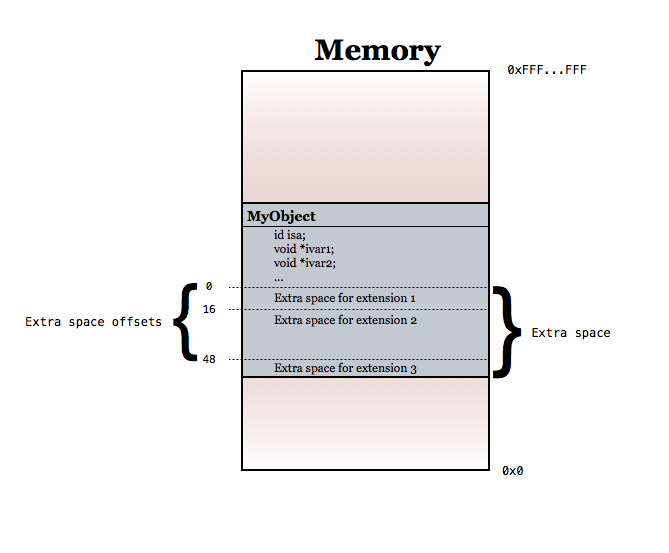
\includegraphics[width=\textwidth]{img/class_extensions.png}
  
  \centering{}
  \caption{Example of how class extensions use memory within an object.}
  \label{fig:class_ext_mem_usage_img}
\end{figure}

While this mechanism allows to extend the classes with new functionality, for example properties, or ARC (the \verb=object_deallocator= can do all the automatic deallocations), it poses an issue at the compile time - how much extra space should be left? The compiler needs to know the size of the class structure (or its prototype to be precise) to generate.

One option is to re-allocate all classes with the extra space and copy over all pointers of the class internal structures (it is enough to copy over pointers as the memory will be kept alive). Assuming 1000 classes in a larger application, each class having 74 bytes (on a 64-bit computer running OS X 10.8), plus those extra bytes, this gives over 64 kB of extra memory per application. While this isn't that much nowadays, it would slow down the application launch and may present a problem when trying to use the run-time on some older or special systems, such as embedded systems.

Other option is to dynamically allocate the extra space for each class, so the class structure stays of the same size, with the extra space being outside of the structure itself. This allows to add class functionality without the compiler support and without recompiling any previous classes (note that this applies only to classes - when allocating objects, we can compute the object size as it is not allowed to add class extensions after the run-time has been initialized).

There are two examples bundled with the run-time: associated objects (see \verb=extras/ao-ext.c=) and categories (see \texttt{extras/categs.c}). Both examples are discussed below the subsection on Performance.

\textbf{Note:} While changing the fields of the class extension that declare the number of extra bytes required is technically possible, after the first object has been allocated, it will not allocate more space. To speed up object allocation, the sum of extra bytes required is cached. Changing these fields will only result in the class extensions reading (or writing over) other extension's memory, and possibly to unallocated memory altogether.

\subsection{Performance}
Just like anything, even adding class extension affects the performance somehow. If no extensions are installed in the run-time, the objects are created directly. If extensions get installed, the extension list needs to be iterated and for each extension, one extra function call is performed, if an object initializing function is installed. This iteration itself doesn't change the asymptotic complexity as the number of class extensions is a constant number, assumed to be a very small one. The only thing that can effect the performance is the object initializer function itself. A quick summary of performance overheads per each function follows.

\begin{itemize}
  \item{\bf{\tt{object\_allocator\_for\_class} and \tt{object\_deallocator\_for\_object}}} The overhead to supplying your own object allocator and deallocator is at least one function call - the run-time needs to call each extension's (de)allocator lookup (this function), if it returns a non-NULL (de)allocator. Assuming that there is only one extension that supplies pieces of memory depending on the instance size passed as the second argument of this function, the overhead is exactly one function, plus the logic within that function.
  \item{\bf{\tt{class\_initializer}}} Common frameworks, such as AppKit and Foundation, include roughly 1000 classes each (which can be verified the aforementioned objc-dump tool), 2000 classes altogether, give or take. Which means 2000 function calls to an initializer for each class extension - per run. As has been mentioned, all of the initialization should be lazy, if possible.
  \item{\bf{\tt{object\_initializer}}} Whenever an object is created, each class extension is given the opportunity to initialize its extra space. Again, all of initialization should be lazy, if possible as there may be many objects allocated that will not take advantage of your particular class extension.
  \item{\bf{\tt{object\_destructor}}} Calling an object destructor is again only calling a function for each class extension. Assuming that number of class extensions is a small and constant number, one can compare such calls to releasing instance variables within the \texttt{dealloc} method - each class extension implementing the destructor would represent one variable.
  \item{\bf{\tt{instance\_lookup\_function} and \tt{class\_lookup\_function}}} These two functions may look like they could present a major slow down as the lookup function should be as fast as possible. This would be true, unless the caching mechanism weren't in place. As has been described above, the run-time first looks into the cache. And only if the method isn't cached, the class extensions are called to look for the implementation, which is really only once per class per method.
\end{itemize}

\subsection{Associated Objects}

Since OS X 10.6, Apple's run-time allows to simulate addition of variables to an object using associated objects\footnote{http://developer.apple.com/library/ios/#documentation/cocoa/conceptual/objectivec/ chapters/ocAssociativeReferences.html}. It allows you to specify an object for a key (which is \verb=void*=). Simply said, each object has a hash map, where it stores objects.

With the class and object extensions, it is fairly easy to achieve. The class itself doesn't need to be modified at all, hence the \verb=class_initializer= may be \verb=NULL= or a no-op function and \verb=extra_class_space= should be set to 0.

The \verb=extra_object_space= can be set to \verb=sizeof(void*)= in case you want to allocate the hash-table structure dynamically, or something else, if you want to inline the structure.

If you want to lazily create the hash-table, the \verb=object_initializer= can be \verb=NULL= or a no-op function as well and the \verb=object_deallocator= should simply deallocate the hash-table structure if it were ever created.

Then you can create some getter and setter functions for associated objects. To access the hash-table from an \verb=id object=, you can use code similar to the following:

\begin{verbatim}
  // Static declaration of the extension
  static objc_class_extension 
      associated_objects_extension = { ... }

  // At the beginning, the extension gets added to the run-time
  objc_class_add_extension(&associated_objects_extension);

  // Hash table is retrieved
  void *hashtable = ((void*)id) + id->isa->instance_size 
        + associated_objects_extension.object_extra_space_offset;
        
  // Do something with the hashtable
\end{verbatim}

\subsection{Categories}



\section{Internal Classes}
\subsection{MRString}

\section{Ports}
\subsection{Windows 3.11}
\subsection{HeSiVa}
